


\section{Why}
\label{sec-1}
In a usual SPH simulation we never track the particles which are in contact
with it.  But suppose say there is a case where we want to have a list of
neighbours which are actually in contact, such as partcicles in its smoothing
length regime.


\section{SPH Example}
\label{sec-2}
I want to discuss two examples to explain the problem here. One is the
simulation of elliptical drop evolution and dam break. These
examples are explainted in terms of pysph implementation.


\subsection{Elliptical drop}
\label{sec-2-1}
To simulate an elliptical drop in PySPH we create an entity with particles
intially at some state. As time evolves they form an elliptical drop.

The code for elliptical drop simulation can be found \href{https://github.com/pypr/pysph/blob/master/pysph/examples/elliptical_drop_no_scheme.py}{here}.

\begin{lstlisting}[language=Python]
 class EllipticalDrop(EDScheme):
     def create_particles(self):
         # code elided
         pa = get_particle_array_wcsph(x=x, y=y, m=m, rho=rho, h=h,
                                     u=u, v=v, name="fluid")

         return [pa]
     # code elided
\end{lstlisting}

So in this simulation we have got one entity with name as \emph{fluid}. So each particle
in this entity can interact any other particle of its own entity.

\subsection{Dam break}
\label{sec-2-2}
Similarly dam break has two entities. Such as "fluid" and "boundary". The
code for simulation can be found \href{https://github.com/pypr/pysph/blob/master/pysph/examples/dam_break_2d.py}{here}. It's a little complicated for our
example.


\begin{lstlisting}[language=Python]
 class DamBreak2D(Application):
     def create_particles(self):
         # Code elided
         fluid, boundary = geom.create_particles(
             nboundary_layers=nboundary_layers, hdx=self.hdx,
             nfluid_offset=nfluid_offset,
         )
         return [fluid, boundary]
     # code elided
\end{lstlisting}

So in this simulation we have got two entity with names as \emph{fluid} and
\emph{boundary}. In this case each particle in fluid can interact with every other
particle in both the entities.


\section{How the data structure looks}
\label{sec-3}
We create a constant for the particle array to save the indices which are in
contact. Let's take a look at the examples to see how this constant can be
formulated.

\subsection{Tracking array in Elliptical drop}
\label{sec-3-1}
Evolution of an elliptical drop can be seen in figure \ref{fig:el_d}.
\begin{figure}[H]
\centering
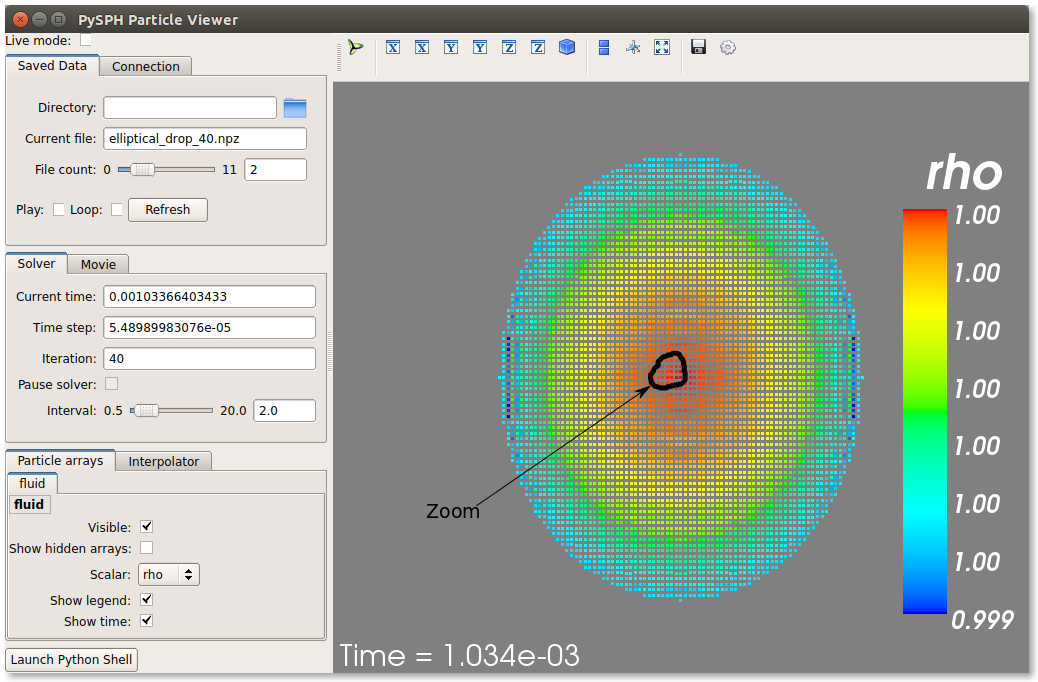
\includegraphics[scale=0.35]{figures/elliptical_drop.png}
\caption{elliptical drop evolution\label{fig:el_d}}
\end{figure}

The particles which are in the influence region of a particle with index
(say 4) can be seen in figure \ref{fig:par_trk_idxs}.

\begin{figure}[H]
\centering
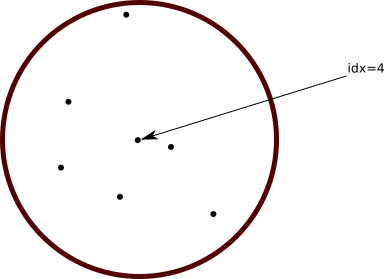
\includegraphics[scale=1]{figures/ed_zoom.png}
\caption{A particle influenced by other particles\label{fig:par_trk_idxs}}
\end{figure}

To keep track of the indices which are in contact, first we assume a maximum
number particles a particle can possible be in a contact with. Let's say 6.

\begin{lstlisting}[language=Python]
     pa.add_constant('limit', 6)
\end{lstlisting}

Now since each particle has a 6 number of neighbours, the constant of trackng
indices would be of a length of total number of particles multiplied by 6 (or
limit).

\begin{lstlisting}[language=Python]
     pa.add_constant('trk_idx', len(pa.x) * limit))
\end{lstlisting}

We can also keep track of number of active contacts which is advantageous
while computing some quantity. This has a length of number of particles.

\begin{lstlisting}[language=Python]
     pa.add_constant('tot_ctcs', len(pa.x))
\end{lstlisting}

\textbf{Note}: Till now we don't have any issues with our 'trk\_idx' array.

Having said that lets move to dam break.

\subsection{Tracking array in Dam break}
\label{sec-3-2}
A typical dam break simulation will look like figure \ref{fig:db}.

\begin{figure}[H]
\centering
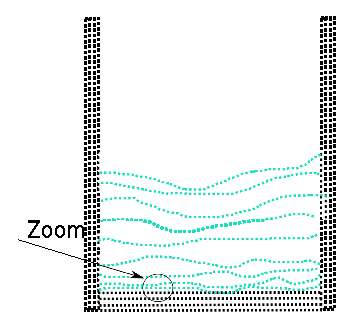
\includegraphics{figures/db.eps}
\caption{Dam break\label{fig:db}}
\end{figure}

When we zoom onto a single fluid particle we can see the particles it is in
contact at that time step, which can be seen in figure
\ref{fig:par_cntct_fluid_boundary}. Now lets see how our 'trk\_idx' looks with
both fluid and solid indices.

\begin{figure}[H]
\centering
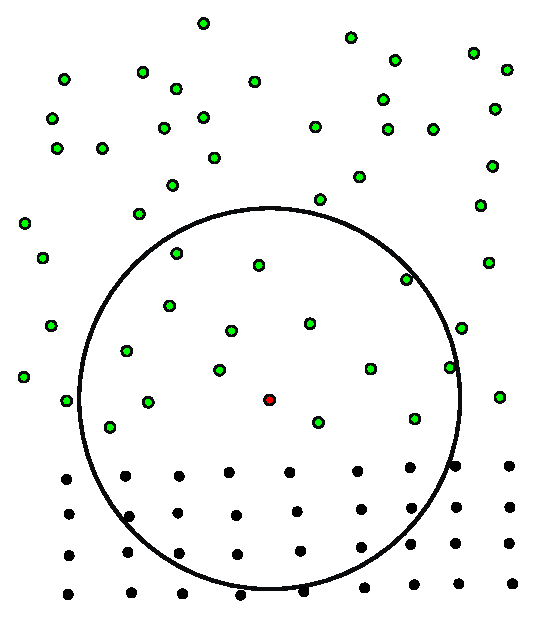
\includegraphics[scale=0.5]{figures/particle_influenced.eps}
\caption{Fluid particle in contact with fluid and boundary\label{fig:par_cntct_fluid_boundary}}
\end{figure}

Since the maximum number of particles a particle can be in contact is defined by \emph{limit}. For a
particle with index \emph{6} the array indices available are

\begin{lstlisting}[language=Python]
     rng_idxs_start = 6 * limit
     rng_idxs_stop = rng_idxs_start + limit
\end{lstlisting}

So every particle will get an array size of \emph{limit}. For a particle with an
index of 6, the array starts at 36 and will end at 41. We are looking at the
indices tracked by the particle in red. The indices could be

\begin{lstlisting}[language=Python]
     trk_idxs = [10, 2, 4, 10, 3, 2, 4]
\end{lstlisting}

We have a \textbf{problem} here. We have repeated indices. Which implies we can't
differentiate which index belongs to which entity. Since the index 10 can
belong to \emph{fluid} or \emph{boundary}.  Same for the rest of the indices.

Worse could be, a particle is actually in contact with fluid with index 2,
but we can assume that it actually belongs to boundary and use boundary
particle properties for any further computation.

To overcome the problem we need to know which index belongs to which particle
array (entity).

\textbf{To be continued\ldots{}}

This problem is solved by using entity id's (Elaborated explanation will be
given later)



\section{Are the tracking indices at a given time are correct?}
\label{sec-4}

\subsection{Simulation at time t0}
\label{sec-4-1}
We are interested in the dynamcis of a system of 5 particles which belong to
the same particle array. At time ($t_0$) the particles look like in figure
\ref{fig:pars_t0_sim}.

\begin{figure}[H]
\centering
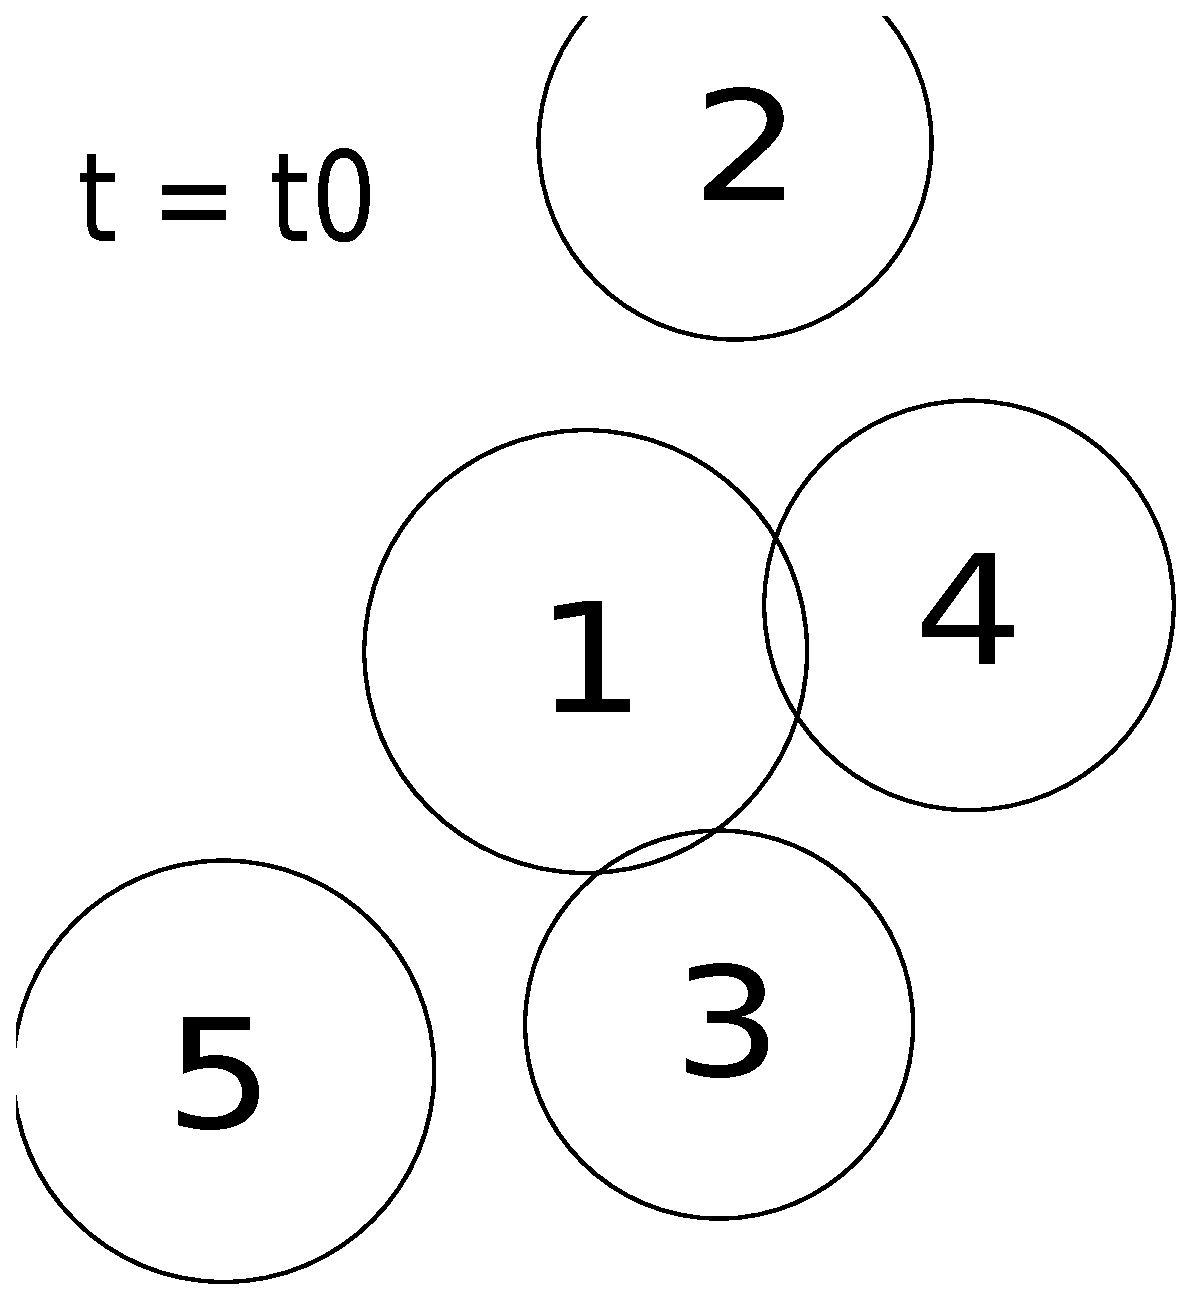
\includegraphics[scale=0.2]{figures/pars_t0.eps}
\caption{Five particles in a simulation\label{fig:pars_t0_sim}}
\end{figure}

Let us focus on the tracking indices of particle 1. Particle with index 1 is
in contact with particles 4 and 5. So the 'trk\_idx' with a limit of 6 would
look like

\begin{lstlisting}[language=Python]
     trk_idxs = [3, 4, -1, -1, -1, -1]
\end{lstlisting}

Now using such information at time ($t_0$) i.e., particles in contact at time t0, we
can compute the forces and other properties of all the particles.

After computation of the force, in the integrator we will move the particles
to next time step. In PySPH that would look like \ref{fig:pars_t0_dt_sim}.
\begin{lstlisting}[language=Python]
      def stage1(self, d_idx, d_x, d_y, d_z, d_u, d_v, d_w, dt):
      d_x[d_idx] = d_x[d_idx] + dt * d_u[d_idx]
      d_y[d_idx] = d_y[d_idx] + dt * d_v[d_idx]
      d_z[d_idx] = d_z[d_idx] + dt * d_w[d_idx]
\end{lstlisting}

Similarly the particles being tracked by particle 1 will also move to the next
time step. Let us say that the particles at time ($t_0+dt$) looks like in figure


\begin{figure}[H]
\centering
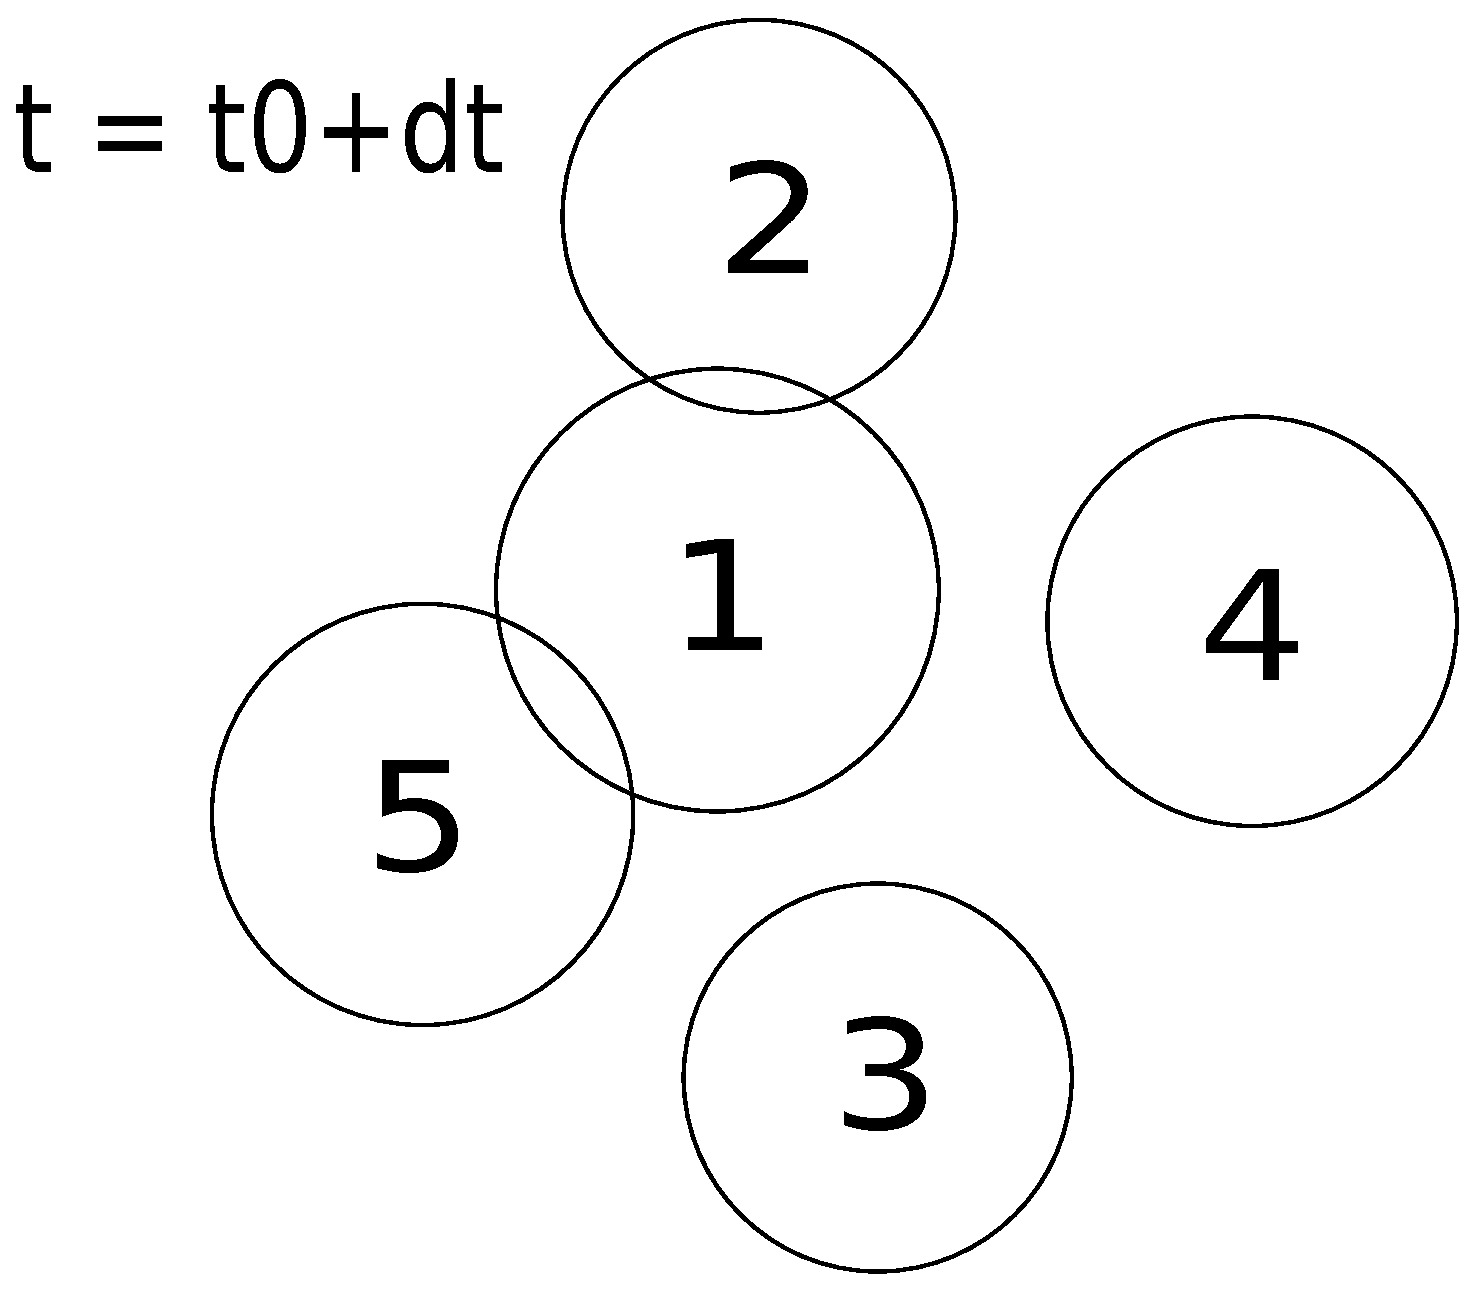
\includegraphics[scale=0.2]{figures/pars_t0_dt.eps}
\caption{Five particles in a simulation\label{fig:pars_t0_dt_sim}}
\end{figure}

\subsection{Simulation at time t0 + dt}
\label{sec-4-2}
Now we are at time $t_0 + dt$. The particles position, velocity other physical
properties are at time $t+t_0$. But \textbf{trk\_idxs} looks like

\begin{lstlisting}[language=Python]
     trk_idxs = [3, 4, -1, -1, -1, -1]
\end{lstlisting}

But it actually should be

\begin{lstlisting}[language=Python]
     trk_idxs = [2, 5, -1, -1, -1, -1]
\end{lstlisting}


\section{How can it be solved?}
\label{sec-5}
One way we could solve it is by executing a equation on the enity with its
sources after completing the time step and update the tracking indices count
with adding new particles. Which would not need any nnps.

\begin{itemize}
\item Either in stage 2 for RK2
\item Or simply a way with which we can execute an equation after completion of a
time step.
\end{itemize}



\section{Why is it important?}
\label{sec-6}
Well we can say that I will adjust the count in the next time step while
computing the force. But that is actually creating a problem with RK2
integrator throught $tang_{x0}$. Since some particles will sure not be in
contact, but $tang_{x0}$ will keep them as they are been tracked at the
initiation of the time step.
% Emacs 25.1.1 (Org mode 8.2.10)
